% !TeX spellcheck = pl_PL
\documentclass[12pt,oneside,a4paper]{article}
\usepackage{polski}
\usepackage{mdwlist}
\usepackage{enumitem}
\usepackage[polish]{babel}
\usepackage[T1]{fontenc}
\usepackage[utf8]{inputenc} 
\usepackage{graphicx}
\usepackage{sidecap}
\usepackage{wrapfig}
\usepackage{indentfirst}
\usepackage{color}
\usepackage{hyperref} 
\hypersetup{
colorlinks=true,
linkcolor=black,
filecolor=magenta,      
urlcolor=cyan,
}
\usepackage{setspace}
\usepackage{blkarray}
\usepackage{longtable}
\usepackage{lipsum}
\singlespacing 
\setlength{\parindent}{25pt}
\setlength{\parskip}{5pt}
\pagestyle{plain}
\usepackage{pdflscape}
\frenchspacing
\widowpenalty=10000
\clubpenalty=10000
\usepackage[tableposition=top]{caption}
\makeatletter

% !TeX spellcheck = pl_PL
\def\TytulPolski    {Projekt zarządzania bezpieczeństwem sieciowego systemu przechowywania danych}

\def\NazwaFirmy {biuro rachunkowe}

\def\Prowadzacy    {mgr inż. Michał Apolinarski}
\def\StudentA     {Maciej Marciniak}
\def\AlbumA       {121996}
\def\EmailA		  {maciej.r.marciniak@student.put.poznan.pl}
\def\StudentB     {Dawid Wiktorski}
\def\AlbumB       {122056}
\def\EmailB		  {dawid.wiktorski@student.put.poznan.pl}

%Kierunek:
\def\Kierunek {Informatyka}
 
%Specjalnosc:
\def\Specjalnosc {Bezpieczeństwo systemów informatycznych} 

%Poziom studiów: 
\def\PoziomStudiow {I stopnia}

%Forma studiów:
\def\FormaStudiow {stacjonarne}  

% Zmiana nazw w opisie tabel i rysunków
\AtBeginDocument{
    \renewcommand*{\tablename}{Tabela}
    \renewcommand*{\figurename}{Rys.} 
}

\makeatletter
\renewcommand\section{\@startsection {section}{1}{\z@}%
	{-3.5ex \@plus -1ex \@minus -.2ex}%
	{2.3ex \@plus.2ex}%
	{\LARGE\scshape\textbf}}
\renewcommand\subsection{\@startsection {subsection}{1}{\z@}%
	{-1.5ex \@plus -1ex \@minus -.2ex}%
	{1.3ex \@plus.2ex}%
	{\large\scshape\textbf}}
\makeatother

\usepackage{multirow}
\usepackage{color}
\usepackage[table]{xcolor}

\begin{document}
	\sloppy
	\thispagestyle{empty}
\begin{center}
Politechnika Poznańska\\
Wydział Elektryczny\\  
Instytut Automatyki i Inżynierii Informatycznej\\
\begin{figure}[ht!]
%\centering
\centering

\includegraphics[width=30mm]{pplogo.png}
\end{figure}
  \LARGE{\TytulPolski}\\ 
   \vspace{5mm}
\end{center}
   \begin{flushright}
   \normalsize\textbf {Twórcy:}\\
\large{\StudentA} \large{\AlbumA}\\
\textcolor{blue}{\large{\EmailA}}\\
\large{\StudentB} \large{\AlbumB}\\
\textcolor{blue}{\large{\EmailB}}\\

\vspace{5mm}
\normalsize\textbf {Właściciele firmy:}\\
\large{Damian Filipowicz} \large{122002}\\
\textcolor{blue}{\large{damian.filipowicz@put.poznan.pl}}\\
\large{Krzysztof Łuczak} \large{122008}\\
\textcolor{blue}{\large{krzysztof.t.luczak@student.put.poznan.pl}}\\
\vspace{3mm}
\large{Specjalność: \Specjalnosc 2017/2018 semestr VII}

\vspace*{\stretch{5}}


prowadzący:\\
\Prowadzacy
\end{flushright}

\begin{center}
Poznań, 2017
\end{center}       	% strona tytułowa
	\newpage\tableofcontents 	  		% spis tresci
	% !TeX spellcheck = pl_PL
\newpage\section*{Wstęp}
\TytulPolski \space polega na zaproponowaniu rozwiązań mających na celu zabezpieczenie systemu, zarządzania nim oraz w jaki sposób przechowywać dane. Zabezpieczaną firmą jest \NazwaFirmy, której właścicielami są Krzysztof Łuczak oraz Damian Filipowicz. 

W pracy najpierw zostanie przedstawiony stan wejściowy firmy, biuro które jest tylko częściowo zabezpieczone przez właścicieli budynku. \linebreak W następnym rozdziale zostanie przeprowadzony audyt bezpieczeństwa, \linebreak mający na celu oszacowanie potencjalnych zagrożeń systemów.

 Następny rozdział przedstawia propozycje przechowania danych. System uwzględnia dostęp do danych poprzez intranet oraz ma mieć na celu minimalizację podatności na uszkodzenia sprzęt.
 
Następnie zostaną zaproponowane zmiany pozwalające poprawić bezpieczeństwo firmy. Kolejnym krokiem jest przeprowadzenie drugiego audytu pozwalającego stwierdzić poziom zagrożeń po wprowadzeniu zmian.

Na koniec zostanie przedstawiony kosztorys wprowadzonych zmian oraz podsumowanie stanu przed i po. 					% wstęp
	% !TeX spellcheck = pl_PL
\newpage\section{Opis zabezpieczanej firmy}
Rozdział zawiera charakterystykę firmy, rodzaj prowadzonej działalności, plan budynku oraz spis sprzętu i pracowników. Jest to stan biura sprzed zabezpieczenia.

\subsection{Charakterystyka firmy}
Firma jest biurem rachunkowym specjalizującym się w doradztwie \linebreak finansowym, prowadzaniu księgowości dla przedsiębiorstw oraz przygotowywaniu analizy finansowej rynku. Przedsiębiorstwo zatrudnia 42 osoby, które tworzą cztery działy: dział ekonomistów, dział sprzedaży, dział IT i dział obsługi.

\subsection{Opis budynku}
Dwupiętrowy budynek firmy zlokalizowany jest na obrzeżach dużego miasta. W okolicy jest pomijalnie niskie ryzyko wystąpienia klęsk \linebreak żywiołowych. Budynek otaczają stare drzewa, których nie można wyciąć, ponieważ objęte są ochroną gatunkową. Do przedsiębiorstwa doprowadzona jest sieć telefoniczna oraz internetowa.

Pomieszczenia w budynku zostały zaprojektowane bez uwzględnienia podłogi technicznej, ani sufitu podwieszanego. Urządzania typu routery (Access Point), switche, kamery, alarmy itp. zostały zamontowane na ścianie lub bezpośredniość w suficie. Przewody zasilające oraz sieciowe poprowadzone są w listwach wzdłuż ścian.

Schemat rozmieszczenie pomieszczeń na parterze i piętrze znajduje się odpowiednio na Rys. \ref{schemat:uklad_pomieszczen_poziom0} i \ref{schemat:uklad_pomieszczen_poziom1}.

\begin{landscape}
	\begin{figure}[!h]
		\vspace{3cm}
		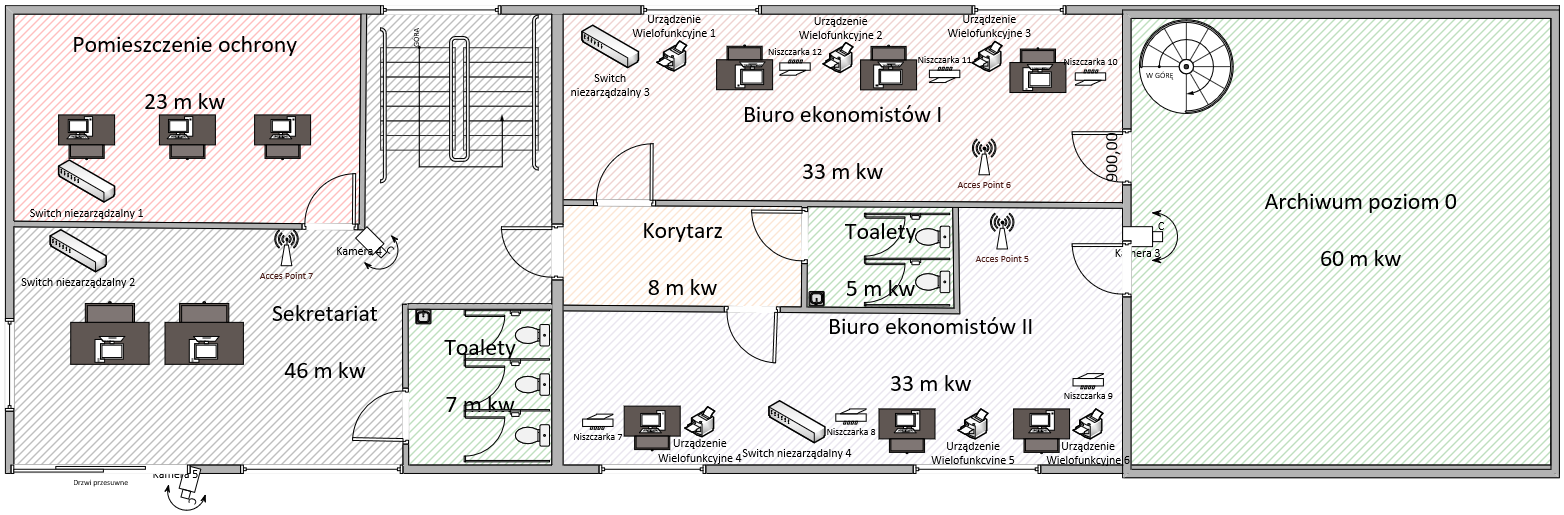
\includegraphics[width=24cm]{uklad_pomieszczen_poziom0.png}
		\caption{Układ pomieszczeń na parterze}
		\label{schemat:uklad_pomieszczen_poziom0}
	\end{figure}
\end{landscape}

\begin{landscape}
	\begin{figure}[!h]
		\vspace{3cm}
		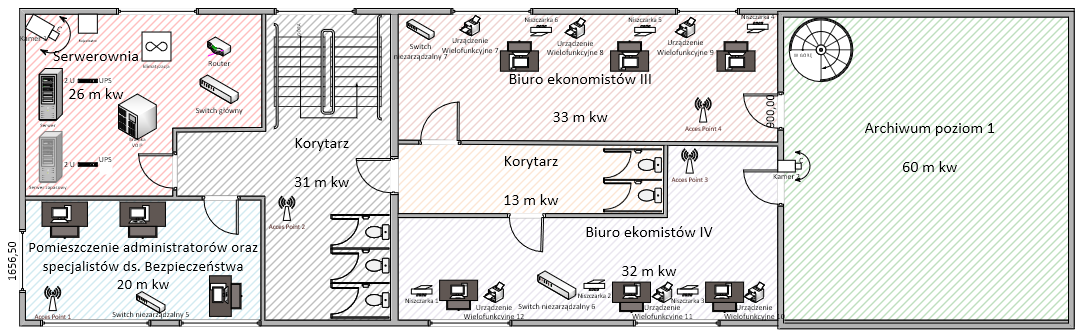
\includegraphics[width=24cm]{uklad_pomieszczen_poziom1.png}
		\caption{Układ pomieszczeń na piętrze}
		\label{schemat:uklad_pomieszczen_poziom1}
	\end{figure}
\end{landscape}

\newpage
\subsection{Organizacja pracy}
W firmie zatrudnionych bezpośrednio jest 32 osób. Dodatkowo 10 osób pochodzi z wynajętych zewnętrznych firm (9 ochroniarzy oraz 1 sprzątaczka). Łącznie w budynku pracuje na zmiany 42 osoby. Biura otwarte są od 6.00 do 22.00, przy czym obowiązują następujące zasady zmian:

\hspace{-0.5cm}\begin{minipage}{13.5cm}
	\begin{itemize*}
		\item Administratorzy pracują w zmianach 6:00-14:00 i 14:00-22:00 \linebreak (po 2 na zmianę),
		\item Specjaliści ds. bezpieczeństwa pracują w zmianach 6:00-14:00 i 14:00-22:00  (po 1 na zmianę),
		\item Ochrona pracuje całodobowo w zmianach 12h z 24h przerwą, pracownicy ochrony zmieniają się w godzinach 4:00 i 16:00(po 3 na zmianę),
		\item Pracownicy sekretariatu pracują od 8:00- 16:00 (po 2 na zmianę),
		\item Dział ekonomistów pracuje w zmianach 6:00-14:00 i 14:00-22:00 \linebreak (po 9 na zmianę),
		\item Dział sprzedaży pracuje w zmianach 6:00-14:00 i 14:00-22:00 \linebreak (po 3 na zmianę),
		\item Sprzątaczka przychodzi w niedzielę, wtorek czwartek o godzinie 22:00.
	\end{itemize*}
\end{minipage}

Pracownicy ochrony podpisują politykę prywatności, mając przy tym dostęp do wszystkich pomieszczeń budynku, wraz z archiwum. Ochroniarz co godzinę po zamknięciu biur przeprowadza obchód po terenie firmy.

Hierarchia pracowników przedstawiona jest na Rys. \ref{schemat:hierarchia_pracownikow}.
\begin{figure}[!h]
	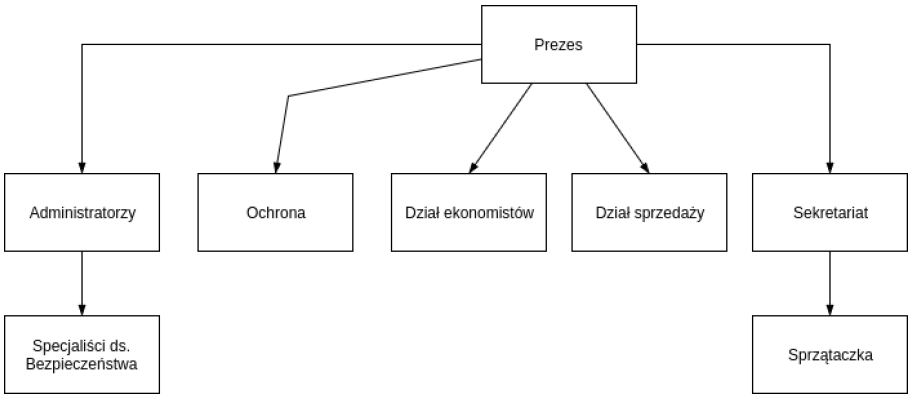
\includegraphics[width=15cm]{Hierarchia_pracownikow.png}
	\caption{Hierarchia pracowników}
	\label{schemat:hierarchia_pracownikow}
\end{figure}
\newpage
\subsection{Sprzęt oraz oprogramowanie}
Poniżej wymieniony został sprzęt informatyczny znajdujący się w firmie wraz z jego podstawowymi parametrami:
\hspace{-0.5cm}\begin{minipage}{13.5cm}
\begin{itemize*}
	\item urządzenie wielofunkcyjne Canon PIXMA G3400 (12 sztuk),
	\item niszczarka ProfiOffice PIRANHA EC 7 CC (12 sztuk),
	\item komputer stacjonarny (18 sztuk):
	\begin{itemize*}
		\item procesor Intel i5,
		\item pamięć 8 GB RAM DDR3,
		\item dysk 1 TB HDD,
		\item myszka, klawiatura, monitor 24",
	\end{itemize*}
	\item laptop DELL Inspiron 5567 (dział IT 6 sztuk),
	\item monitor ochrony 24" (2 sztuki),
	\item telefon VoIP Cisco CP-7940G (17 sztuk),
	\item serwer główny (1 sztuka):
	\begin{itemize*}
		\item płyta główna: Intel S2600CP4,
		\item procesor Intel Xeon e5-2603 v2,
		\item pamięć 128 GB RAM DDR3,
		\item dyski SSD o łącznej pojemności 40 TB, 
	\end{itemize*}
	\item serwer zapasowy (1 sztuka):
	\begin{itemize*}
		\item płyta główna: Intel S2600CP4,
		\item procesor Intel Xeon e5-2603 v2,
		\item pamięć 16 GB RAM DDR3,
		\item dyski SSD o łącznej pojemności 10 TB, 
	\end{itemize*}
	\item router Cisco RV325 (1 sztuka),
	\item switch główny Cisco SG300-52 (1 sztuka),
	\item bramka VoIP Grandstream HT704 (1 sztuka),
	\item switch niezarządzalny Cisco SB SF100D-16EU (7 sztuk),
	\item punkt dostępowy Asus RP-AC87 (7 sztuk),
	\item okablowanie:
	\begin{itemize*}
		\item między serwerami skrętka kategorii SF/FTP 7A (40 Gb/s),
		\item pozostałe połączenia skrętka  kategorii U/UTP 6 (200 Mb/s),
	\end{itemize*}
	\item UPS VOLT Micro 1200 (1 sztuka),
	\item monitoring:
	\begin{itemize*}
		\item rejestrator BCS-P-QDVR0801ME z dyskiem 2 TB HDD (1 sztuka),
		\item kamera LV-IP2301IP (5 sztuk),
	\end{itemize*}
	\item taśmy magnetyczne.
\end{itemize*}
\end{minipage}

\newpage
Poniżej znajduje się spis oprogramowania (licencji) jakie jest \linebreak zainstalowane w komputerach:

\hspace{-0.5cm}\begin{minipage}{13.5cm}
\begin{itemize}
	\item komputery pracowników w dziale ekonomistów:
	\begin{itemize}
		\item Windows 10 (9 sztuk),
		\item pakiet Office 2016 (9 sztuk),
		\item pakiet Insert GT (9 sztuk),
		\item Windows Defender (9 sztuk),
	\end{itemize}
	\item komputery sekretariatu, ochrony i działu sprzedaży:
	\begin{itemize}
		\item Windows 10 (6 sztuk),
		\item pakiet Office 2016 (6 sztuk),
		\item Windows Defender (6 sztuk),
	\end{itemize}
	\item komputery pracowników w dziale IT:
	\begin{itemize}
		\item Windows 10 (6 sztuk),
		\item pakiet Office 2016 (6 sztuk),
		\item pakiet Insert GT (6 sztuk),
		\item Windows Defender (6 sztuk),
	\end{itemize}
	\item oprogramowanie serwera i wykorzystywane technologie:
	\begin{itemize}
		\item Linux Ubuntu 16.04 LTS z OpenStack (umożliwia wirtualizację
		\linebreak dowolnego systemu),
		\item bazy danych MSSQL,
		\item bazy danych MySQL,
		\item OpenVPN,
		\item Windows Server 2016 (5 sztuk),
		\item Pakiet Insert GT (5 sztuk),
		\item system pocztowy Exim i Dovecot: Roundcube jako klient poczty \linebreak w przeglądarce.
	\end{itemize}
\end{itemize}
\end{minipage}

\newpage
\subsection{Schemat sieci informatycznej}
Sieci informatyczna składa się z routera do którego podłączony jest \linebreak Internet (poprzez światłowód), switcha głównego, 7 switchy niezarządzanych, centrali VoIP oraz 7 punktów dostępowych. Schemat sieci przedstawiony jest na Rys. \ref{schemat:schemat_sieci_infor}. Oznaczenie trzech kropek symbolizuje możliwość podpięcia wielu urządzeń do sieci.

\begin{landscape}
\begin{figure}[!h]
	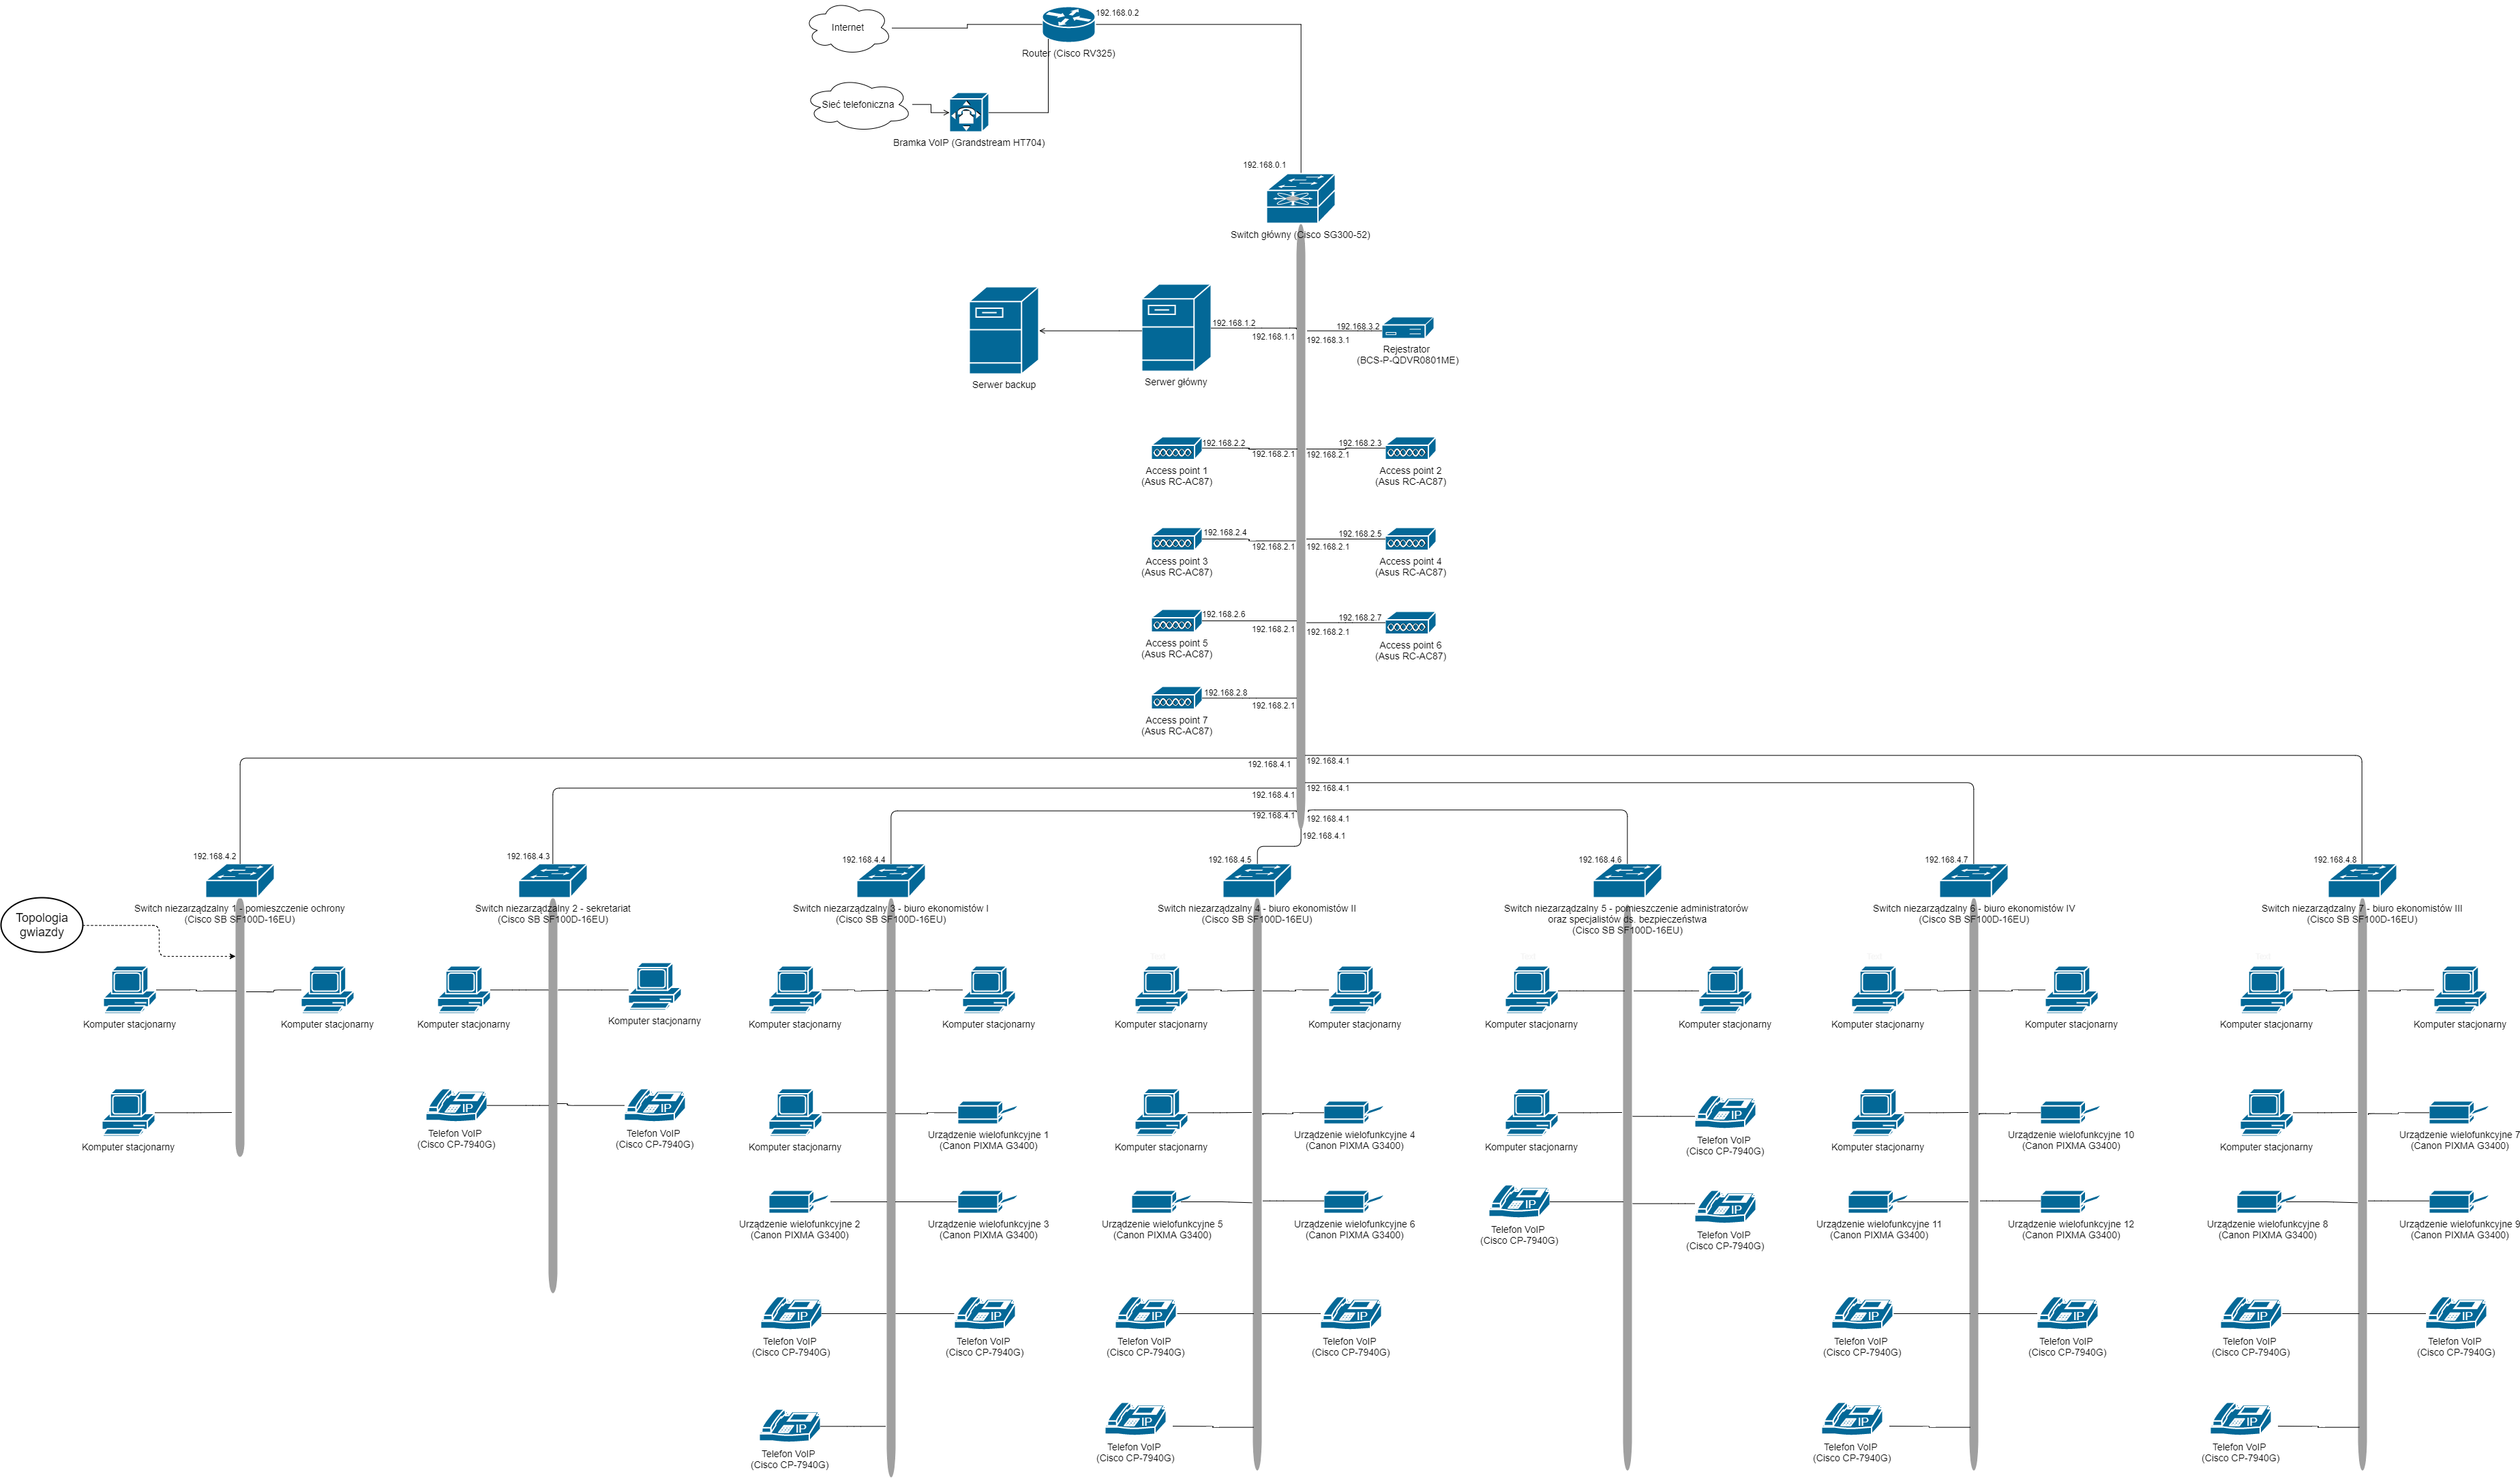
\includegraphics[width=24cm]{Schemat_sieci.png}
	\caption{Schemat sieci informatycznej}
	\label{schemat:schemat_sieci_infor}
\end{figure}
\end{landscape}

\newpage
\subsection{Przechowywane dane}
Przechowywane dane użytkowe znajdują się na dyskach twardych \linebreak w komputerach oraz na serwerze. Pliki archiwalne oraz kopie zapasowe umieszczone zostają na dyskach serwerowych oraz starsze dane na taśmach magnetycznych w celu obniżenia kosztów. Do przechowywanych danych \linebreak należą:

\hspace{-0.5cm}\begin{minipage}{13.5cm}
	\begin{itemize*}
		\item Dane finansowe klientów - pliki PDF, DOCX, pliki specyficzne dla programu Insert GT, bazy danych,
		\item Dane personalne klientów,
		\item Nagrania z monitoringu (miesiąc wstecz),
		\item Kopia zapasowa:
		\begin{itemize*}
			\item Kompresowana,
			\item Codziennie różnicowa dla danych klientów (raz w tygodniu pełna),
			\item Codziennie przyrostowa dla monitoringu,
			\item Codziennie pełna kopia konfiguracji urządzeń,
		\end{itemize*}
		\item Dane zatrudnienia oraz księgowość firmy.
	\end{itemize*}
\end{minipage}

Wszystkie przechowywane dane mają charakter informacji wrażliwych, ponieważ firma głównie operuje na danych osobowych. Dane finansowe klientów maja charakter tajny, ze względu na niebezpieczeństwo wykorzystania tych informacji przez nieprzyjazną konkurencję.

Szacowany przyrost danych:

Tygodniowy przyrost danych oscyluje w okolicach 1 GB danych + kopia zapasowa około 500 MB. Kopia danych klientów z ostatniego roku trzymana jest na serwerze backupu. Kopie dalsze znajdują się na taśmach magnetycznych w archiwum - dodatkowo te, które tego wymagają są drukowane. Dane w archiwum przechowywane są przez 5 lat po tym okresie dane są przenoszone do osobnego archiwum, którym zajmuje się zewnętrzna firma.
          	% opis firmy
	% !TeX spellcheck = pl_PL
\newpage\section{Identyfikacja zagrożeń \newline i analiza ryzyka}
W niniejszym rozdziale zostanie przeprowadzony audyt bezpieczeństwa. Zostaną przedstawione potencjalne zagrożenia w systemie oraz zdefiniowana zostanie metoda oceny ryzyka.

\subsection{Ocena ryzyka - metoda jakościowa}
Do oceny ryzyka wykorzystano metodę jakościową OWASP Risk Rating Methodology. W zależności od wpływu oraz prawdopodobieństwa wystąpienia zagrożenia, określa się jakie ze sobą niesie ryzyko. 
\begin{table}[!ht]
	\centering
	\caption{Ocena ryzyka}
	\label{ocenaRyzyka}
	\begin{tabular}{|c|c|c|c|c|}
		\hline 
		\multicolumn{5}{|c|}{Ryzyko}        \\ \hline
		\multirow{4}{*}{} & Wysoki  & \cellcolor{orange} Średnie     &\cellcolor{red}  Wysokie   & \cellcolor{pink} Krytyczne     \\ \cline{2-5} 
		Wpływ	  & Średni  & \cellcolor{yellow} Niskie    	 & \cellcolor{orange} Średnie    & \cellcolor{red}  Wysokie   \\ \cline{2-5}
		& Niski   & \cellcolor{green} Bardzo niskie &  \cellcolor{yellow} Niskie     & \cellcolor{orange} Średnie    \\ \cline{2-5}
		&     	& Niskie   			& Średnie    &  Wysokie    \\ \hline
		& \multicolumn{4}{c|}{Prawdopodopieństwo}  \\  \hline 
	\end{tabular}
\end{table}

\subsection{Potencjalne zagrożenia}
W tym podrozdziale opisane zostaną potencjalne zagrożenia oraz w tabelach zostanie ocenione ryzyko jakie niosą ze sobą dane niebezpieczeństwa. Zagrożenia podzielono na trzy kategorie: zagrożenia naturalne, zagrożenia ludzkie oraz zagrożenia techniczne.

\subsubsection{Zagrożenia naturalne} 
Zagrożenia naturalne.
Zagrożenia naturalne związane są z lokalizacją przedsiębiorstwa, należą do nich:
	\begin{itemize*}
		\item zanik prądu,
		\item upadek drzewa,
		\item pożar.
	\end{itemize*}
Wymienione zagrożenia mają wpływ na dostępność danych. W budynku nie ma systemu przeciwpożarowego, a więc podczas pożaru, wysoka temperatura może uszkodzić sprzęt. Również uszkodzenie sprzętu może nastąpić w czasie zaniku prądu. Zasilacze awaryjne (UPS) podczas braku prądu dostarczają energię elektryczną tylko do serwerów i pozostały sprzęt jest narażony na uszkodzenie. W tabeli 2. oceniono ryzyko związane z zagrożeniami naturalnymi.
\begin{table}[!ht]
	\centering
	\caption{Zagrożenia naturalne}
	\label{zagrożeniaNaturalne}
	\begin{tabular}{|c|c|c|c|}
		\hline
		\textbf{Podatność} & \textbf{Prawdopodobieństwo} & \textbf{Wpływ} & \textbf{Ryzyko} \\ \hline
		Zanik prądu        & Niskie                      & Średni         & Niskie          \\ \hline
		Upadek drzewa      & Niskie                      & Średni         & Niskie          \\ \hline
		Pożar              & Niskie                      & Wysoki        & Średnie         \\ \hline
	\end{tabular}
\end{table}

\subsubsection{Zagrożenia ludzkie}
To na dole jest do zrobienie :)  \\
Jednym z zagrożeń jest możliwość upadku drzewa na budynek firmy, co może spowodować pożar lub utratę prądu. W przypadku pożaru istnieje duże ryzyko utraty danych (wpływ na dostępność danych), ponieważ żadne z~pomieszczeń nie posiada systemu przeciwpożarowego.  Prawdopodobieństwo wystąpienia upadku drzewa na budynek obecnie jest stosunkowo niskie. Natomiast, trzeba wziąć pod uwagę zmieniający się klimat w Polsce, który w~przyszłości będzie sprzyjał powstawaniu silnych wiatrów, a tym samym prawdopodobieństwo wystąpienia tego zjawiska będzie coraz większe. \\ \colorbox{yellow}{Wpływ - średni, prawdopodobieństwo - niskie, ryzyko - niskie.}

Następnym zagrożeniem jest włamanie się do budynku. Zadanie nie jest trudne, ponieważ w oknach nie są stosowane alarmy, zamki na klucz czy też kraty, które utrudniłyby dostanie się do budynku. Również, drzwi nie są specjalnie zabezpieczone, a więc włamywacz przy pomocy, np. wytrychu jest w stanie w łatwy sposób dostać się do każdego pomieszczenia. Prawdopodobieństwo wystąpienia fizycznego włamania do budynku jest na średnim poziomie. Skutki mogą być poważne. Włamywacz nie tylko może ukraść sprzęt/dane (zagrożenie zasad poufności danych), ale także może zainstalować oprogramowanie szpiegujące lub zmodyfikować istniejące dane (wpływ na zasady integralności danych). \\ \colorbox{orange}{Wpływ - wysoki, prawdopodobieństwo - średnie, ryzyko - wysokie.}

W komputerach pracowników używany jest Windows Defender, który nie jest tak skuteczny przeciwko wirusom jak produkty konkurencji. W przypadku gdy, użytkownik pobierze zainfekowany plik, istnieje średnie prawdopodobieństwo, że zawirusowany zostanie komputer, czy też inne urządzenia podłączone do sieci (naruszenie zasad integralności oraz poufności). \\ \colorbox{orange}{Wpływ - wysoki, prawdopodobieństwo - średnie, ryzyko - wysokie.}

Hackerzy mają ułatwione zadanie związane z dostaniem się na serwery dlatego, że w serwerach nie jest używane dodatkowe oprogramowanie związane z bezpieczeństwem (złamanie zasady poufności oraz wysokie zagrożenie integralności danych). Nie ma też sprzętowej zapory ogniowej, która filtrowałaby cały ruch sieciowy. \\ \colorbox{pink}{Wpływ - wysoki, prawdopodobieństwo - wysokie, ryzyko - krytyczne.}

Firma nie jest odpowiednio przygotowana na spadki napięcia lub zanik prądu, ponieważ w czasie awarii zasilania wszystkie komputery, kamery \linebreak razem z rejestratorem obrazu i inne urządzenia elektryczne wyłączą się. Nagłe wyłączenie się komputerów może spowodować utratę ważnych danych lub też uszkodzenie komponentów w komputerze (wysoki stopnień naruszenia zasad dostępności oraz integralności). Wyłączenie się kamer utrudnia ochronę budynku. Zasilacze awaryjne (UPS) dostarczają energię elektryczną tylko do serwerów. \\ \colorbox{red}{Wpływ - wysoki, prawdopodobieństwo - średnie, ryzyko - wysokie.}

Brak wystarczającej ilości kamer, aby odpowiednio monitorować budynek z zewnątrz i wewnątrz. Kamery przy wejściu do budynku i w sekretariacie na parterze mają zbyt dużą powierzchnię do monitorowania, co powoduje istnienie martwych pól przez długi czas. Wówczas poruszając się poza widocznością kamery można włamać się (skutki zostały opisane wcześniej). 

Monitory obrócone w stronę okna umożliwiają podejrzenie co dana osoba wykonuje na komputerze, zatem naruszona zostaje poufności przeglądanych materiałów. \\ \colorbox{yellow}{Wpływ - średni, prawdopodobieństwo - niskie, ryzyko - niskie.}

Brak polityki bezpieczeństwa powoduje sytuację, w której użytkownicy mogą używać prostych haseł, czy też przez długi okres czasu nie zmieniać ich. Uruchomiony odpowiedni program może złamać takie hasła niezależnie od skomplikowania hasła, również hasło może być poznane w stosunkowo krótkim czasie, czy będzie trywialne. Uzyskanie dostępu do sytemu przez nieupoważnione osoby spowoduje naruszenie zasady poufności. Osoba taka może również zmienić hasło użytkownika, co ograniczy dostępność do zasobów, można również zmodyfikować dane naruszając integralność. \\  \colorbox{red}{Wpływ - wysoki, prawdopodobieństwo - wysokie, ryzyko - krytyczne.}

Niezabezpieczone porty USB umożliwiają użytkownikowi nie tylko kopiowanie danych z firmy, ale również zainfekowanie komputera, czy też jego uszkodzenie przy użyciu np. USB Killer (zagrożenie dla poufności danych, dostępności oraz integralności). \\ \colorbox{pink}{Wpływ - wysoki, prawdopodobieństwo - wysokie, ryzyko - krytyczne.}

Nieużywanie programów do blokowania instalacji programów ułatwia użytkownikowi wgranie dowolnego oprogramowania. Bez blokowania  dostępu do wybranych stron internetowych, użytkownicy mogą wchodzić na strony zainfekowane (zgrożenie dla poufności danych i integralności). \\ \colorbox{orange}{Wpływ - wysoki, prawdopodobieństwo - niskie, ryzyko - średnie.} 

Bezpieczeństwo poczty elektronicznej jest zapewnione przez używanie odpowiedniego oprogramowania. Natomiast, komunikacja w celu wysłania pliku między komputerami lub między komputerem a drukarką nie jest zabezpieczona. Istnieje więc ryzyko zmodyfikowania pliku, bądź też jego przejęcia przez nieautoryzowaną osobę  (zagrożenie dla poufności danych i integralności). \\   \colorbox{orange}{Wpływ - wysoki, prawdopodobieństwo - niskie, ryzyko - średnie.}  

Kolejnym zagrożeniem jest topologia sieci internetowej, a konkretniej połączenie poprzez sieć bezprzewodową. Istnieje możliwość wykorzystania sieci otwartej WiFi do przedostania się do innych podsieci, a nawet \linebreak w~skrajnym przypadku do serwerów (naruszenie poufności oraz integralności danych). Również niebezpieczeństwem \linebreak związanym z siecią jest brak alternatywnego połączenia z Internetem (brak zapewnienia dostępności). \\ \colorbox{red}{Wpływ - wysoki, prawdopodobieństwo - średnie, ryzyko - wysokie.}


% uwzględnić rodzaj danych: tajne, ściśle tajne, wrazliwe
% wyszczególnić wpływ zagrożenia na poufność, dostepność i itegralność
% sprecyzować prawdopodobieństwo ryzyka
% 
					% opis audytu przed zabezpieczeniem systemu
	% !TeX spellcheck = pl_PL
\newpage
\section{System przechowywania \newline danych}
Rozdział ten przedstawia propozycję systemu przechowywania danych. Struktura sieci informatycznej jest rozbudowana, zatem aby scentralizować dostęp do danych zastosowano technologię NAS.

\subsection{Struktura NAS}
Dostęp do serwera NAS nie wymagają telefony IP oraz bramka VoIP, zatem nie zostały uwzględnione w strukturze. Schemat systemu NAS znajduje się na rysunku \ref{schemat:schemat_sieci_NAS}. Połączenia pomiędzy stacjami roboczymi poprowadzone są poprzez iSCSI (wykorzystując sieć przewodową).
\begin{landscape}
	\hspace{4cm}
	\begin{figure}[!h]
		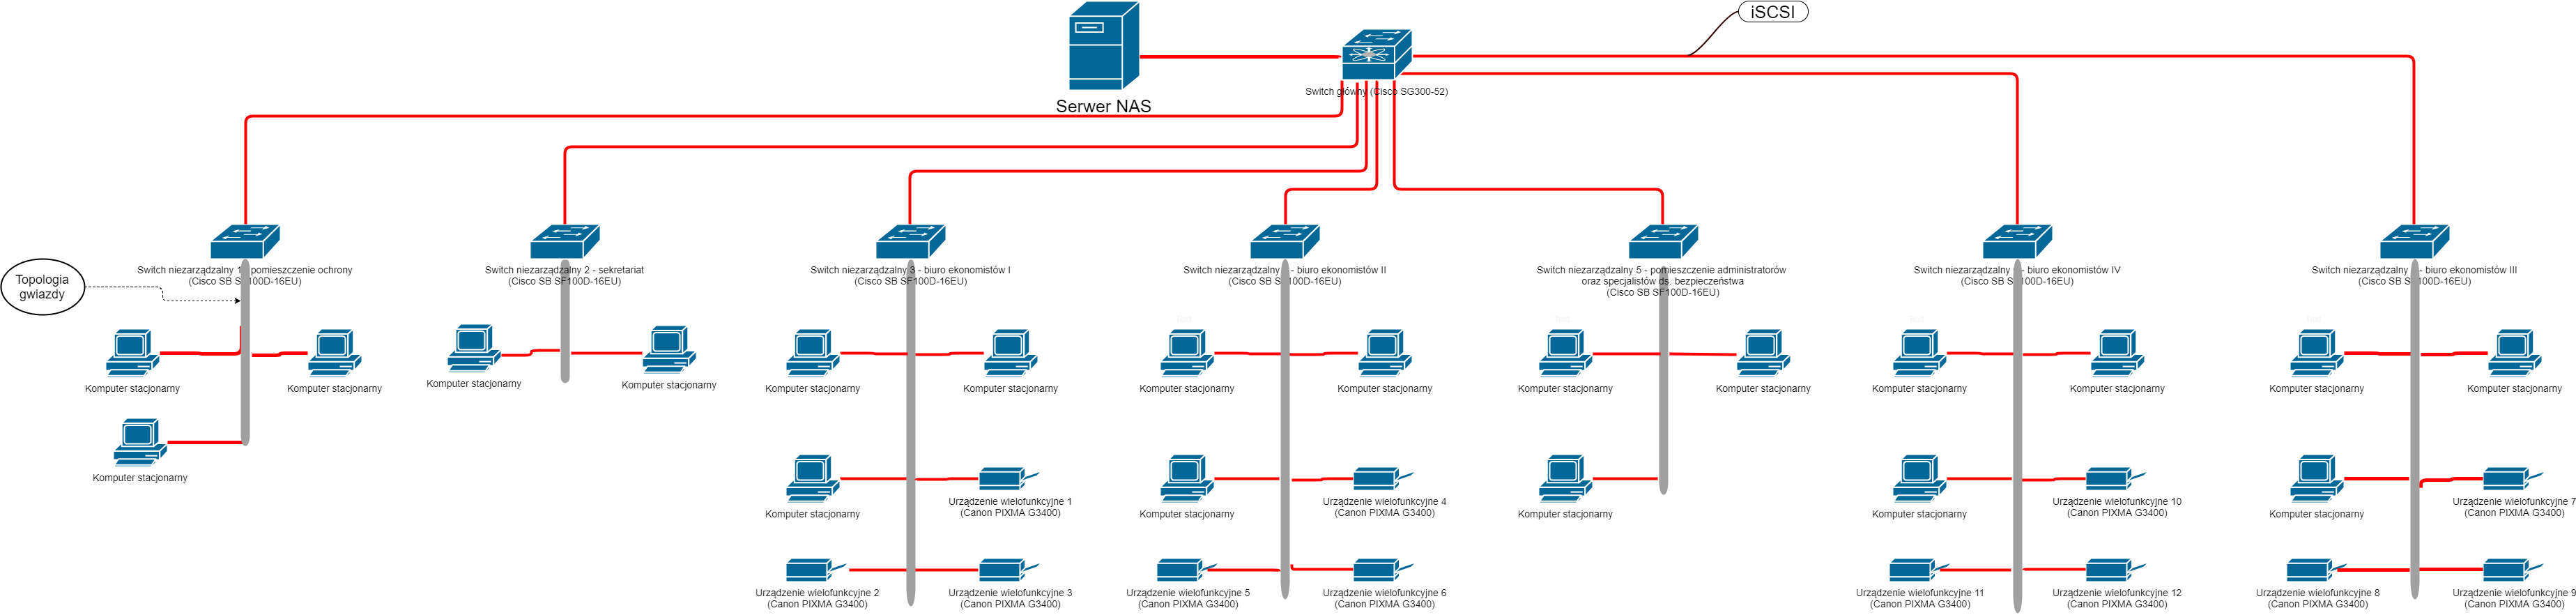
\includegraphics[width=24cm]{Schemat_NAS.png}
		\caption{Schemat struktury NAS}
		\label{schemat:schemat_sieci_NAS}
	\end{figure}
\end{landscape}

\subsection{Serwer}
Serwer główny ze względu na potrzebę niezawodności pracy posiada macierz dyskową RAID 4 z 3 dyskami HDD WD Red 2TB. W przypadku awarii dowolnego dysku istnieje możliwość odtworzenia utraconych danych. Jest to wolniejsze rozwiązanie niż powiedzmy RAID 5, ale zapewnia większe bezpieczeństwo w przypadku uszkodzenia. Wykorzystując daną macierz dyskową posiadamy 4TB pojemności dyskowej, wg podanych informacji od zleceniodawców taki rozmiar pamięci powinien wystarczyć na przechowywanie danych przez 50 lat (jest to okres przez jaki należy przechowywać dane księgowe).

Serwer zapasowy posiada kompletną kopię macierzy dyskowej z serwera głównego zapewniając redundancję w przypadku całkowitej awarii sprzętu. W~ten sposób zabezpieczamy w znacznym stopniu dane przed utraceniem.

Na serwerze w środowisku wirtualnym uruchomiony jest system FreeNAS odpowiedzialny za zarządzanie przechowywaniem plików. W systemie FreeNAS uruchomione są usługi odpowiedzialne za replikację danych oraz tworzenie kopii zapasowych. Pełna kopia zapasowa będzie wykonywana w każdy poniedziałek, natomiast kopia przyrostowa będzie wykonywana w pozostałe dni tygodnia. Każda kopia zapasowa będzie szyfrowana algorytmem AES.

Dodatkowo kopie zapasowe z okresu powyżej roku przechowywane są na taśmach magnetycznych w pomieszczeniu archiwum.

\subsection{Komputery pracowników}
Komputery pracowników ze względu na nie zbyt wysoką szkodliwość utraty danych (pod warunkiem przenoszenia danych systematycznie do pamięci serwera - NAS) nie wymagają szczególnych zabezpieczeń. Wykorzystano dwa rodzaje dysków: HDD WD Black 500GB dla plików oraz SSD Samsung 850 Pro 120GB dla wybranych programów oraz systemu operacyjnego. W przypadku braku dwóch slotów dyskowych drugi dysk (HDD) zastępuje napęd optyczny. Magistralą użytą w komputerach jest SATAIII ze względu na parametry techniczne komputerów (brak magistrali NVIe).


\section{Trwałe usuwnaie danych}
Na nośnikach danych w postaci dysków twardych i taśm magnetycznych przechowywane są wrażliwe dane osobowe oraz dane dotyczące przedsiębiorstwa. Aby, takie dane nie trafiły w niepowołane ręce podczas wymiany sprzętu czy też jego awarii, należy zadbać o bardzo ważny aspekt jakim jest trwałe usunięcie danych z nośników. Wyróznia się dwie metody usuwania danych: programową oraz sprzętową. W przypadku, gdy nośnik jest sprawny, zaleca się użycie odpowiedniego programu (Acronis Drive Cleanser), który w sposób bezpieczny trwale usunie dane. Taka metoda usuwania danych jest nie tylko tańsza, ale też skuteczniejsza i bezpieczniejsza dla środowiska niż metoda fizyczna. Metodę sprzętową zaleca się używać, gdy nośnik danych jest niesprawny. Jedną z najbardziej skutecznych metod fizycznych usuwania danych jest wykorzystanie wysokiej temperatury powyżej 1000 stopni Celsjusza. Przy poprawnym procesie usuwania za pomocą odpowiedniej temperatury, nie da się odczytać danych w warunkach domowych i laboratoryjnych.
	% opis systemu przechowywania danych
\end{document}